\documentclass[tikz,border=10pt]{standalone}
\usepackage[T1]{fontenc}
\usepackage[utf8]{inputenc}
\usepackage{lmodern}
\usepackage{amsmath,amssymb}
\usetikzlibrary{arrows.meta,positioning,shapes.geometric,calc}
\definecolor{jac}{HTML}{73539E}
\definecolor{ink}{HTML}{354052}
\tikzset{
 >=Stealth,
 state/.style={draw=jac,fill=jac!7,rounded corners=5pt,align=center,minimum width=26mm,minimum height=11mm,inner sep=5pt,font=\small},
 action/.style={state,fill=white},
 decision/.style={draw=jac,fill=jac!7,diamond,aspect=2.4,inner sep=1.8pt,align=center,font=\small},
 success/.style={state,draw=teal!75!black,fill=teal!7},
 failure/.style={state,draw=red!70!black,fill=red!5},
 arrow/.style={->,thick,draw=ink},
 note/.style={align=left,font=\footnotesize,text=ink}
}
\begin{document}

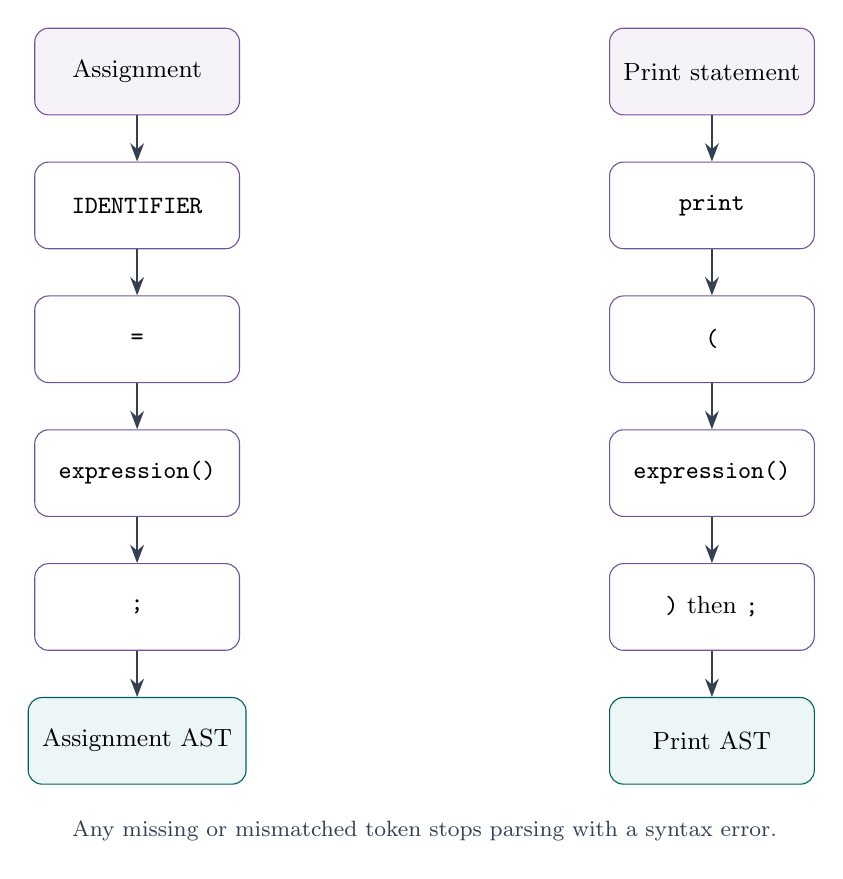
\begin{tikzpicture}[font=\small]
\node[state] (a0) at (0,0) {Assignment};
\node[action] (a1) at (0,-1.7) {\texttt{IDENTIFIER}};
\node[action] (a2) at (0,-3.4) {\texttt{=}};
\node[action] (a3) at (0,-5.1) {\texttt{expression()}};
\node[action] (a4) at (0,-6.8) {\texttt{;}};
\node[success] (a5) at (0,-8.5) {Assignment AST};
\node[state] (p0) at (7.3,0) {Print statement};
\node[action] (p1) at (7.3,-1.7) {\texttt{print}};
\node[action] (p2) at (7.3,-3.4) {\texttt{(}};
\node[action] (p3) at (7.3,-5.1) {\texttt{expression()}};
\node[action] (p4) at (7.3,-6.8) {\texttt{)} then \texttt{;}};
\node[success] (p5) at (7.3,-8.5) {Print AST};
\foreach \a/\b in {a0/a1,a1/a2,a2/a3,a3/a4,a4/a5,p0/p1,p1/p2,p2/p3,p3/p4,p4/p5} \draw[arrow] (\a)--(\b);
\node[note,below=9mm of $(a5)!0.5!(p5)$] {Any missing or mismatched token stops parsing with a syntax error.};
\end{tikzpicture}

\end{document}
